\chapter{Test on Simulation of RC Vehicle}\label{chap:test-chronos}

In this chapter, we present the test of the safety filter introduced in \cref{chap:robust-ddsf-lti} on the simulation of an RC vehicle.
We will first introduce the vehicle model and simulation setup, including the simplified kinematic model and the more realistic dynamic model.
We also discuss the design and choice of terminal ingredient for this model, and briefly discuss how can we evaluate the performance of the safety filter.
Then the result for kinematic model will be presented, showing that for this simple non-linear model, the indirect formulation of robust safety filter introduced in \cref{sec:indirect-formulation} can successfully guarantee safety, even when the output is noisy.
Finally, we present the result for the dynamic model, showing that the robust safety filter can also guarantee safety for this more realistic model, when we have access to the noise-free output.


\section{Vehicle Model and Simulation Setup}\label{sec:model-sim-setup}

In this section we introduce the vehicle model and simulation setup used in this chapter.
Our model is based on the RC vehicle \emph{Chronos}, and its simulation/control framework \emph{CRS} as introduced in \cite{carronChronosCRSDesign2022}.

\subsection{Vehicle Model}\label{subsec:vehicle-model}

We have two different models for the vehicle, the simplified kinematic model and the more realistic dynamic model, as introduced in \cite{carronChronosCRSDesign2022} by (1)-(4) and (5) and (6), respectively.
They are both based on global coordinates, which is the most general and convenient for model-based controllers and safety filters.
For example, the model is successfully used for the design of the safety filter in \cite{tearlePredictiveSafetyFilterRacing2021}.

However, for the data-driven predictive safety filter, we need to find an equilibrium of the system, and the system will be operating around this equilibrium.
This global coordinate model does not guarantee such a good equilibrium.

In contrast, the track-relative coordinates introduced in \cite{tearlePredictiveSafetyFilterRacing2021} is more suitable for the data-driven predictive safety filter.
We can also design different equilibrium for track-relative coordinates, as will be introduced in \cref{sec:result-kinematic-model}.

As can be seen in \cref{fig:track-relative-coordinates}, the track-relative coordinates are defined for a certain piece of track, with $\elat$ being the deviation of vehicle from the centerline, and $\mu$ being the difference of heading angle from the tangent of the centerline.

\includefig{error-dynamics.pdf}{0.5}{Track-relative coordinates}{fig:track-relative-coordinates}

The dynamic model in track-relative coordinates is given by (6), (7) and (11) in \cite{tearlePredictiveSafetyFilterRacing2021}, we only introduce the kinematic model here:

\begin{subequations}
\label{eq:kinematic-model}
\begin{gather}
    x = \begin{bmatrix}
        \elat \\
        \mu \\
        v \\
        l
    \end{bmatrix} 
    , \; u = \begin{bmatrix}
        \tau \\
        \delta
    \end{bmatrix} \label{eq:kinematic-state} \\
    \dot{x} = \begin{bmatrix}
        v \sin\left(\mu + \beta\right) \\
        \frac{v}{l_r} \sin\left(\beta\right) - c \frac{v \cos\left(\mu + \beta\right)}{1 - c \elat} \\
        \frac{\tau}{m} \\
        \frac{v \cos\left(\mu + \beta\right)}{1 - c \elat}
    \end{bmatrix}
    , \; \beta = \atangent\left(\frac{l_r}{l_r + l_f} \tan(\delta)\right) \label{eq:kinematic-dynamics}
\end{gather}
\end{subequations}

where $x$ is the state, $u$ is the input, $m$, $l_f$ and $l_r$ are the mass, front and rear length of the vehicle, respectively, $c$ is the curvature of the track.

\subsection{Simulation Setup}\label{subsec:simulation-setup}

In general, the track on which the vehicle is driving can be complicated, and the curvature $c$ can be varying.
For simplicity, we only work with track with piece wise constant curvature, of width $w=\SI{0.5}{m}$.

In practice, the constraint \emph{``the vehicle should not leave the track''} can be complicated to formulate, considering the vehicle shape \cite{tearlePredictiveSafetyFilterRacing2021}.
In this chapter, to simplify the problem, we view the vehicle as a point of mass, and the constraint is simplified to $-\frac{w}{2} \leq \elat \leq \frac{w}{2}$.
We also impose a constraint on the heading angle $\mu$: $-\frac{\pi}{2} \leq \mu \leq \frac{\pi}{2}$, to avoid the vehicle from driving backwards.
We use a numerical ode solver CVODE \cite{gardner2022sundials} via the CasADi \cite{AnderssonCasadi2019} interface to simulate the vehicle.
The sampling time is set to $\SI{0.01}{s}$.
The optimization problem is solved by MOSEK \cite{mosek}.
For the kinematic model, we set the output of system to $\transpose{\begin{bmatrix}\elat & \mu & v\end{bmatrix}}$, for the dynamic model, it will be $\transpose{\begin{bmatrix}\elat & \mu & \vx & \vy\end{bmatrix}}$.
More specific setups, including other parameters, constraints, initial conditions, hyperparameters for the safety filter, and scheme for choosing leaning based inputs, will be introduced in the corresponding sections.


\section{Design of Terminal Ingredient}\label{sec:design-terminal-ingredient}

Before we present the result for the safety filter, we need to discuss the design and choice of terminal ingredient for the vehicle model.
Note that, although this design process takes usage of the \emph{formulation} of the vehicle dynamics, it does not require any knowledge of the \emph{parameters} of the vehicle dynamics.

Within the scope of this Thesis, we set the terminal constraint to an equilibrium of the system, so the question is reduced to finding an equilibrium of the system.

For the vehicle model, we can find the following schemes to find an equilibrium:

\paragraph{Fitting for Constant $\elat$ and Velocity}
As can be seen from the kinematic model, if we set $\elat$ and $v$ to be constant, the system will implicitly be in equilibrium.
However, without further knowledge about the system parameters, it is hard to find the value of $\mu$ and $\us$ corresponding to a given $\elat$ and $v$.
We can use the dataset and \cref{lemma:fundamental-lemma} to fit for the value of $\mu$ and $\us$ corresponding to a given $\elat$ and $v$:

\begin{equation}\label{eq:fitting-equilibrium}
    \vRepeatVec{\ys}{L} = \Yf \pinv{\hankeluyone} \begin{bmatrix}
        \vRepeatVec{\us}{l} \\
        \vRepeatVec{\us}{L} \\
        \vRepeatVec{\ys}{l} \\
        1
    \end{bmatrix}
\end{equation}

By fixing $\elat$ and $v$ in $\ys$, we can infer a linear system from \cref{eq:fitting-equilibrium} and solve it for $\mu$ and $\us$.

\paragraph{Fixing $\mu$ and Velocity in Optimization Problem}
Another observation is, if the heading angle $\mu$ and velocity $v$ are fixed, the system will implicitly be in equilibrium.
Although it is also possible to fit other variables similarly in \cref{eq:fitting-equilibrium}, here we choose another method to find the equilibrium.
Similar to the method in \cite{mullerDataDrivenQCR2022}, where the equilibrium is implicitly defined and decided by the predictor, we can also let the optimization problem decide the equilibrium.
In the terminal constraint, only the velocity is constrained to be a certain constant.
The heading angle $\mu$, deviation from centerline $\elat$, and steering angle $\delta$ is constrained to be the same for the last $n$ time steps, but the specific value is not constrained.

\paragraph{Stopping at a Certain Point}
As we are dealing with a vehicle, a natural choice of terminal constraint is to stop the vehicle at a certain point.
We can choose to stop the vehicle at a certain point, for example on the centerline, or let it stop anywhere on the track.
As for the constraint, we can constrain the velocity to be zero for the last $n$ steps, and we can set other constraints as we like, for example we can constrain the deviation from centerline to be zero.

We implemented all the methods mentioned above to the kinematic model, with some model-specific design add (for example in some cases we can fix the throttle $\tau_s = 0$).
And the results are presented and discussed in \cref{sec:result-kinematic-model}.
For the dynamic model, we only use the ``Fixing $\mu$ and Velocity in Optimization Problem'' method, and the result is presented and discussed in \cref{sec:result-dynamic-model}.


\section{Simulation Using Kinematic Model}\label{sec:result-kinematic-model}

In this section, we present the result for the safety filter on the kinematic model.
For the dataset and online observation, we set the noise level to $\SI{1}{\milli\meter}$ for position on both $x$ and $y$ axis, $\SI{0.01}{\radian}$ for heading angle, and $\SI{0.005}{\meter/\second}$.
Each noise is sampled from a uniform distribution with the given range.
Here we present the result with objective input as maximum throttle $\tau_{\max}$ and sine wave steering input.
The terminal ingredient is chosen to be the ``Fixing $\mu$ and Velocity in Optimization Problem'' method.
Also, we choose a prediction horizon of $L = 150$, corresponding to $\SI{1.5}{\second}$.
The number of input-output pairs used for initial condition is set to $l = 15$.
The constraint tightening is set to a list of $[0.25, 0.1, 0.05, 0.01] \times w/2$ for $\elat$ and $[0.1, 0.1, 0.05, 0.01] \times 0.5 \pi$ for $\mu$.
We use a dataset of length $N = 1000$ for each curvature.
The dataset is collected by simulating the system for $1000$ time steps, starting from the equilibrium of system $\ys$, and applying a random input added by the equilibrium input $\us$.
The equilibrium $\us$ and $\ys$ is found by solving a non-linear equation.
This dataset collection process designed to collect a dataset close to the designed equilibrium, but is not realistic in practice, since it uses knowledge of the system parameters.
However, it is still useful for testing the safety filter, as it is a good approximation of the real dataset, and it is easy to collect.
In practice, we can use manual input to keep the system around the equilibrium when collecting the dataset.

\begin{figure}[ht]
    \centering
    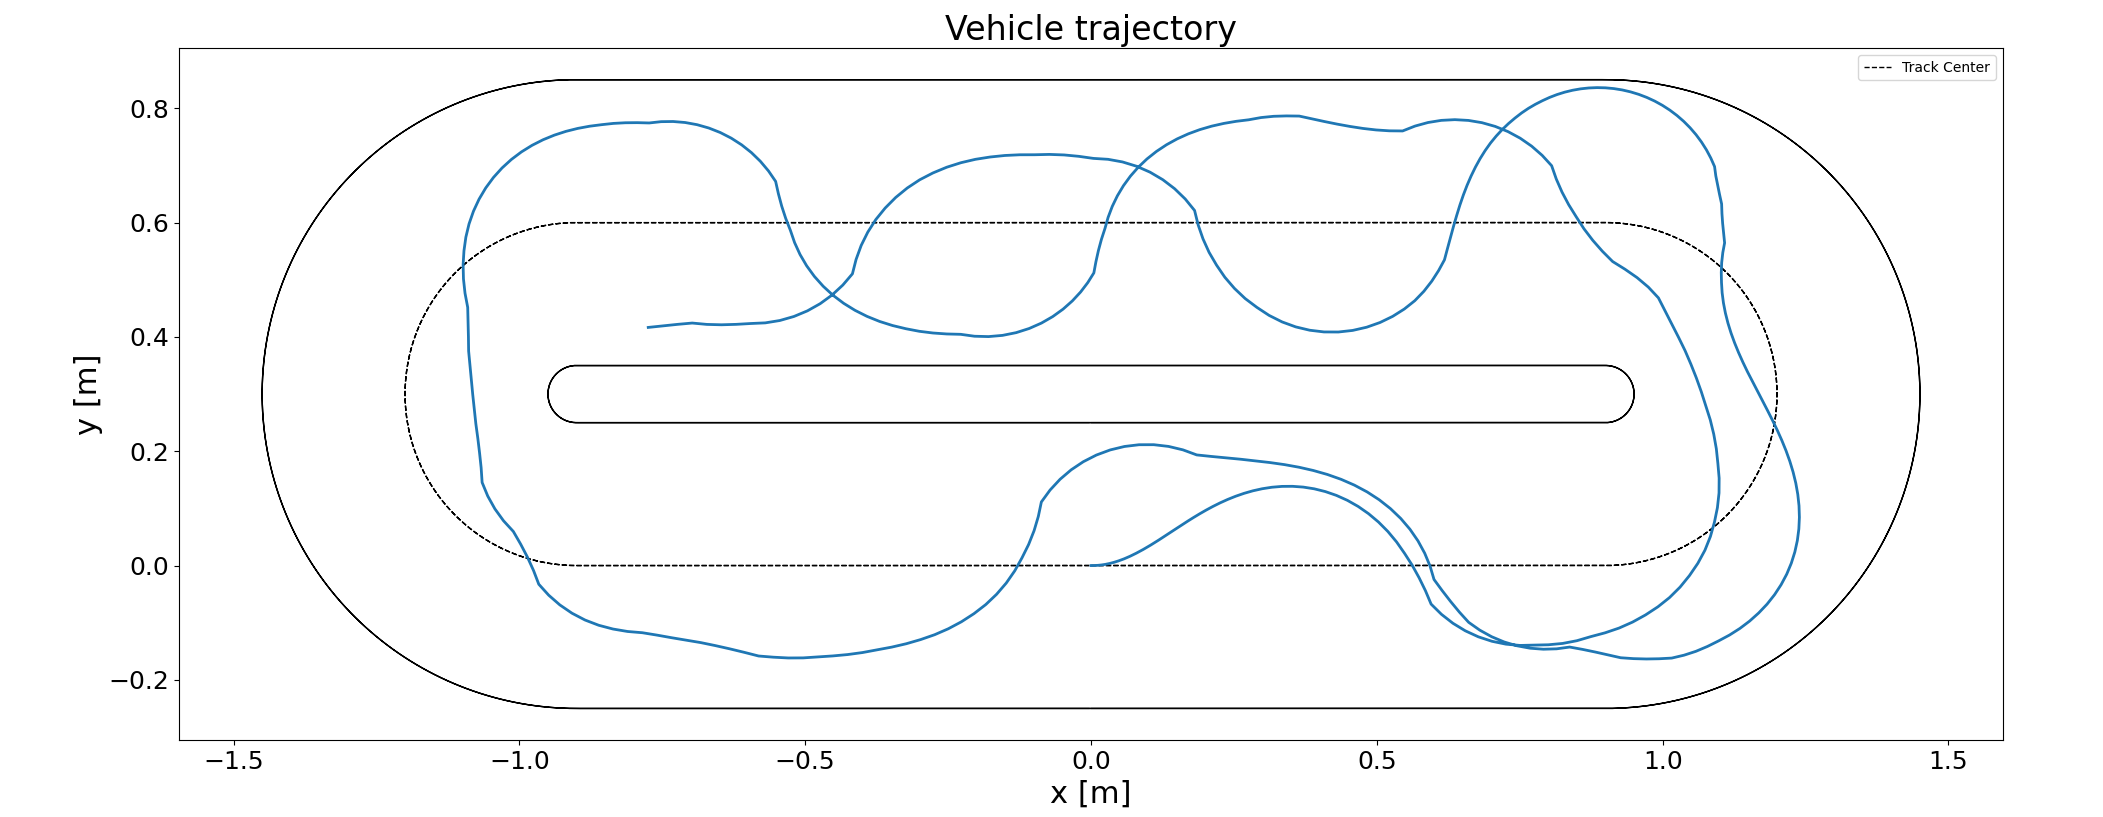
\includegraphics[width=0.9\textwidth]{\imagedir/kinematic-trajectory.png}
    \caption{Trajectory of the vehicle, the blue line being the trajectory}
    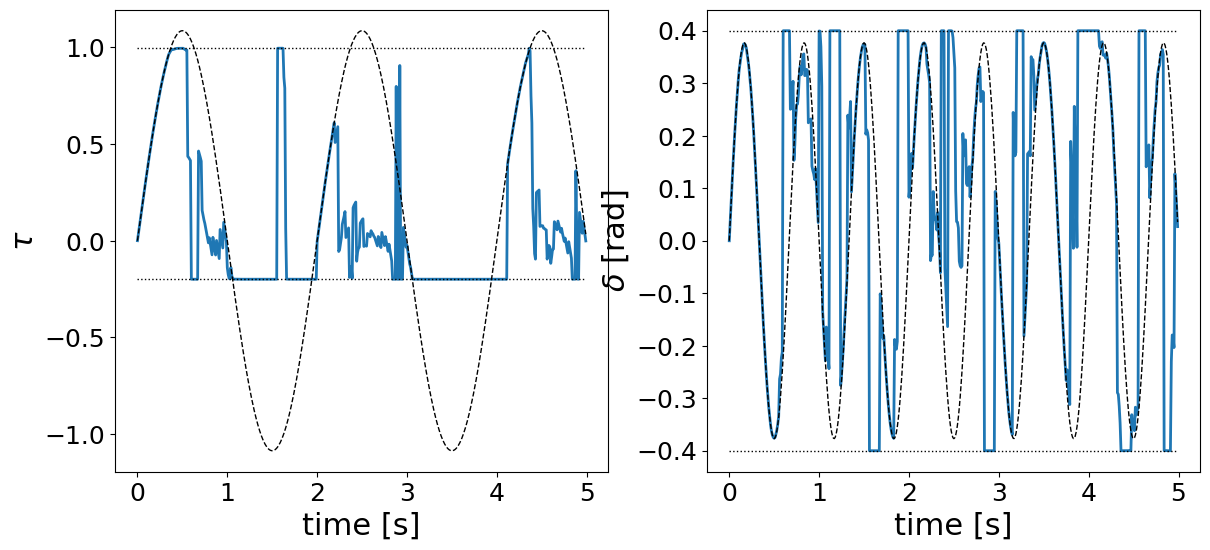
\includegraphics[width=0.9\textwidth]{\imagedir/kinematic-sin-sin-inputs.png}
    \caption{Objective and applied inputs, the dotted line being the objective input and blue line being the applied input}
    \label{fig:kinematic-single-run}
\end{figure}

We can see from \cref{fig:kinematic-single-run}, the objective inputs are modified by the safety filter and it successfully keeps the vehicle on the track.

We also present the result of applying different terminal ingredients, as mentioned in \cref{sec:design-terminal-ingredient}.
Here the objective input is set to full throttle $\tau_s = \tau_{\max}$.
The hyperparameters are adjusted for each terminal ingredient.
To avoid the hyperparameters to overfit to this specific objective control, they are tuned so to make sure that the vehicle can successfully drive around the track with three different objective control input rules, including `Max Throttle with Zero Steering', `Max Throttle with Sine Steering' and `Sine Throttle with Sine Steering'.

\begin{figure}[ht]
    \centering
    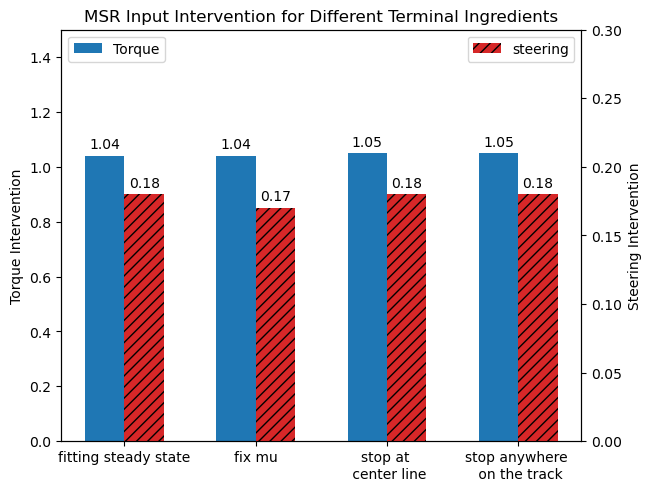
\includegraphics[width=0.7\textwidth]{\imagedir/kinematic-terminal-comparison.png}
    \caption{Input interference for different terminal ingredients}
    \label{fig:kinematic-terminal-comparison}
\end{figure}

We can see from \cref{fig:kinematic-terminal-comparison} that, with finely tuned hyperparameters, all the terminal ingredients have very similar mean squared input interference.

It's worth noting that, it's not necessary true that smaller mean squared input interference means better performance for a safety filter.
For example, a safety filter can have smaller mean squared input interference by always modifying the input to some point, so the vehicle can always stay near the centerline.
While another safety filter will only make large interference when the vehicle is about to leave the track, resulting in a larger mean square input interference.
However, the second safety filter is more desirable, as it will not interfere with the vehicle when it is driving normally.
There are no good metrics to evaluate the performance of a safety filter yet, and we will not discuss this topic further in this Thesis.


\section{Simulation Using Dynamic Model}\label{sec:result-dynamic-model}

This section presents the result for the safety filter on the dynamic model.
As stated before, we only use the ``Fixing $\mu$ and Velocity in Optimization Problem'' method to find the terminal ingredient.

Also, we assume we have noise-free access to the output, both in the dataset and online observation.
We take use of the prediction method introduced in \cref{chap:non-linear-system} to make predictions for the dynamic model.
The prediction horizon is set to $L=80$, number of input-output pairs used for initial condition set to $l=10$, and the constraint tightening constants being: $[0.25, 0.1, 0.05, 0.01] \times \elat_{\max}$, $[0.2, 0.1, 0.05, 0.01] \times \mu_{\max}$, $[0.2, 0.1, 0.05, 0.01] \times \vx_{\max}$, and $[0.1, 0.05, 0.01, 0.005] \times \vy_{\max}$, for the corresponding four outputs.
For the prediction method, we choose $Q$ so that all the input/outputs are normalized by the corresponding maximum value, and the weighting function $w(d) = \frac{1}{d}$.
Similar to the case in \cref{sec:non-linear-system-numerical-example}, we only use the trajectory slices that are close enough to current initial state, if enough number of such slices are available.

Before the simulation, a dataset trajectory of length $N=1000$ is collected, by a similar method in \cref{sec:result-kinematic-model}.
In addition, we introduce a scheme of collecting more dataset with a more realistic method, as can be seen in \cref{fig:data-collection-process}.

\includefig{data-collection-process.png}{0.7}{The process of dataset collection, each run uses a different controller or objective input scheme, and stops after safe constraint not satisfied}{fig:data-collection-process}

In this framework, in addition to the dataset collected by the method in \cref{sec:result-kinematic-model}, we also collect online-data starting from a realistic initial condition and realistic objective input, which does not use knowledge of the system parameters.
Here in the dataset collection runs, we set the objective input to be a sine wave with randomly chosen frequency and phase.
As can be seen from \cref{fig:data-collection-process}, At each iteration a data-collection process is conducted, and the dataset is updated.
After that, in application runs, the new dataset is used for the safety filter.
We do not directly use dataset from the application runs, to avoid the weighting method putting too much weight onto several trajectory slices that are very close to current state.
This can be a problem, when at each iteration the same controller or objective input is applied, as the system will travel along a very similar trajectory.
For this certain example, in the application runs, we apply three different kinds of open loop objective input, as introduced in \cref{sec:result-kinematic-model}.

As the final result, after two iterations, the safety filter is able to keep the vehicle within the track boundaries for all application runs.
Here we present the trajectory and inputs with the objective input being `Sine Throttle with Sine Steering', as can be seen in \cref{fig:dynamic-single-run}.


\begin{figure}[ht]
    \centering
    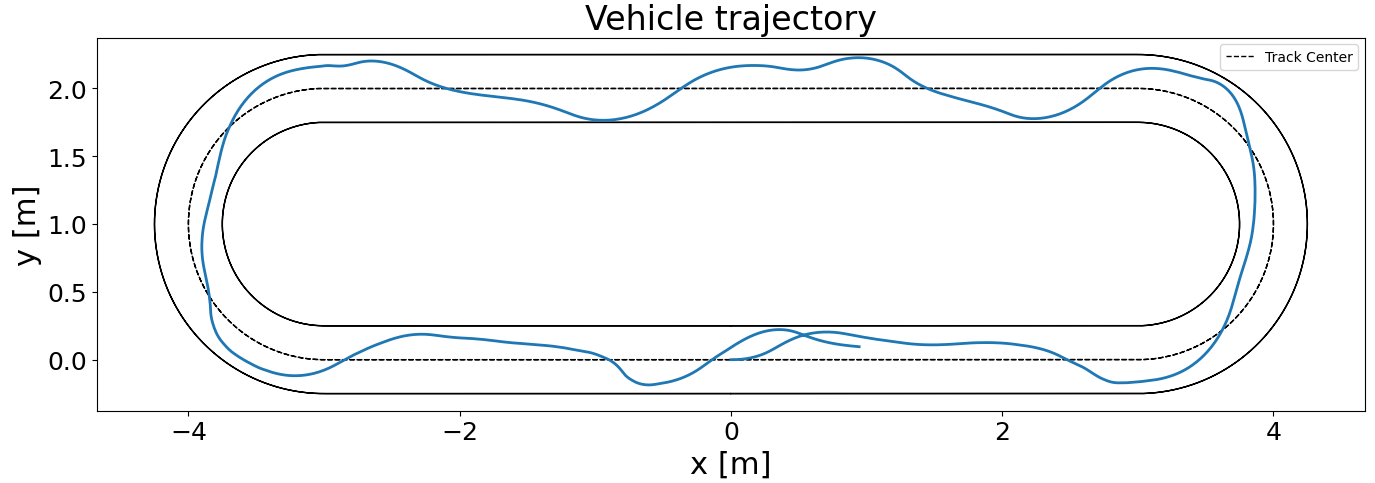
\includegraphics[width=0.9\textwidth]{\imagedir/dynamic-sin-sin-trajectory.png}
    \caption{Trajectory of the vehicle, the blue line being the trajectory}
    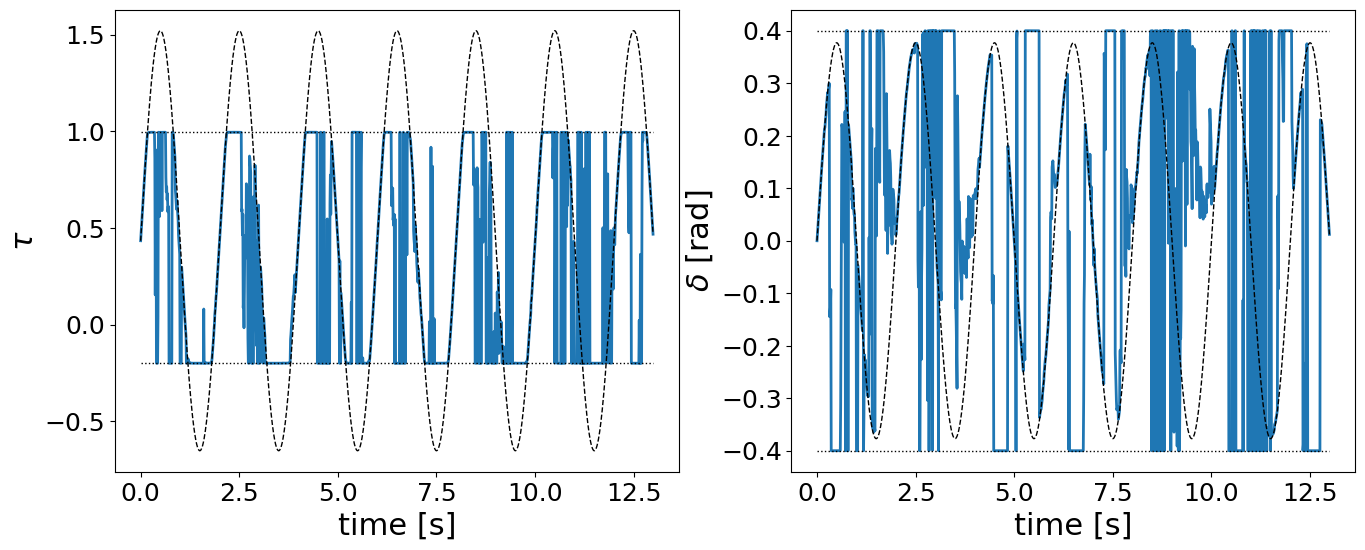
\includegraphics[width=0.9\textwidth]{\imagedir/dynamic-sin-sin-inputs.png}
    \caption{Objective and applied inputs, the dotted line being the objective input and blue line being the applied input}
    \label{fig:dynamic-single-run}
\end{figure}

We can see from \cref{fig:dynamic-single-run}, the safety filter is able to keep the vehicle within the track boundaries, even with the more realistic dynamic model.
There are still many improvements to be made for the safety filter, though.
For example, the resulting input sequence is not smooth, and can not be applied to the real RC vehicle.
Also, similar improvements mentioned for the prediction method in \cref{sec:weighting-method} can also be applied to the safety filter.
